\subsection{Implementation}
Our networks and loss functions are implemented using built-in TensorFlow
functions \cite{TensorFlow}, enabling us to use automatic differentiation for all gradient
computations. To make our code easy to extend and flexible, we build on
the TensorFlow Object detection API \cite{TensorFlowObjectDetection}, which provides a Faster R-CNN baseline
implementation.
On top of this, we implemented Mask R-CNN and the Feature Pyramid Network (FPN)
as well as the Motion R-CNN extensions for motion estimation and related evaluations
and postprocessings. In addition, we generated all ground truth for
Motion R-CNN in the form of TFRecords from the raw Virtual KITTI
data to enable fast loading during training.
Note that for RoI extraction and bilinear crop and resize operations,
we use the \texttt{tf.crop\_and\_resize} TensorFlow function with
interpolation set to bilinear.

\subsection{Datasets}
\label{ssec:datasets}

\paragraph{Virtual KITTI}
The synthetic Virtual KITTI dataset \cite{VKITTI} is a re-creation of the KITTI
driving scenario \cite{KITTI2012, KITTI2015}, rendered from virtual 3D street
scenes.
The dataset is made up of a total of 2126 frames from five different monocular
sequences recorded from a camera mounted on a virtual car.
Each sequence is rendered with varying lighting and weather conditions and
from different viewing angles, resulting in a total of 10 variants per sequence.
In addition to the RGB frames, a variety of ground truth is supplied.
For each frame, we are given a dense depth and optical flow map and the camera
extrinsics matrix. There are two annotated object classes, cars, and vans (N$_{cls}$ = 2).
For all cars and vans in each frame, we are given 2D and 3D object bounding
boxes, instance masks, 3D poses, and various other labels.

This makes the Virtual KITTI dataset ideally suited for developing our joint
instance segmentation and motion estimation system, as it allows us to test
different components in isolation and progress to more and more complete
predictions up to supervising the full system on a single dataset.

For our experiments, we use the \emph{clone} sequences, which are rendered in a
way that most closely resembles the original KITTI dataset. We sample 100 examples
to be used as validation set. From the remaining 2026 examples,
we remove a small number of examples without object instances and use the resulting
data as training set.

\paragraph{Motion ground truth from 3D poses and camera extrinsics}
We will now describe how we use the ground truth poses and camera matrices from Virtual KITTI to
compute instance and camera motion ground truth.
For two consecutive frames $I_t$ and $I_{t+1}$,
let $[R_t^{ex}|t_t^{ex}]$
and $[R_{t+1}^{ex}|t_{t+1}^{ex}]$
be the camera extrinsics at the two frames.
We compute the ground truth camera motion
$\{R_{cam}^*, t_{cam}^*\} \in \mathbf{SE}(3)$ as

\begin{equation}
R_{cam}^* = R_{t+1}^{ex}  \cdot \mathrm{inv}(R_t^{ex}),
\end{equation}
\begin{equation}
t_{cam}^* = t_{t+1}^{ex}  - R_{cam}^* \cdot t_t^{ex}.
\end{equation}

Additionally, we define $o_{cam}^* \in \{ 0, 1 \}$,
\begin{equation}
o_{cam}^* =
\begin{cases}
1 &\text{if the camera pose changes between $t$ and $t+1$} \\
0 &\text{otherwise,}
\end{cases}
\end{equation}
which specifies whether the camera is moving in between the frames.

For any object $k$ visible in both frames, let
$(R_t^k, t_t^k)$ and $(R_{t+1}^k, t_{t+1}^k)$
be its orientation and position in camera space
at $I_t$ and $I_{t+1}$, respectively.
Note that the pose at $t$ is given with respect to the camera at $t$ and
the pose at $t+1$ is given with respect to the camera at $t+1$.

We define the ground truth pivot $p_k^* \in \mathbb{R}^3$ as
\begin{equation}
p_k^* = t_t^k
\end{equation}
and compute the ground truth object motion
$\{R_k^*, t_k^*\} \in \mathbf{SE}(3)$ as
\begin{equation}
R_k^* = \mathrm{inv}(R_{cam}^*) \cdot R_{t+1}^k \cdot \mathrm{inv}(R_t^k),
\end{equation}
\begin{equation}
t_k^* = t_{t+1}^{k}  - R_k^* \cdot t_t^k.
\end{equation}

As for the camera, we define $o_k^* \in \{ 0, 1 \}$,
\begin{equation}
o_k^* =
\begin{cases}
1 &\text{if the position of object i changes between $t$ and $t+1$} \\
0 &\text{otherwise,}
\end{cases}
\end{equation}
which specifies whether an object is moving in between the frames.

\paragraph{Evaluation metrics with motion ground truth}
To evaluate the 3D instance and camera motions on the Virtual KITTI validation
set, we introduce a few error metrics.
Given a foreground detection $k$ with an IoU of at least $0.5$ with a ground truth example,
let $R_k, t_k, p_k, o_k$ be the predicted (and postprocessed) motion for the predicted class $c_k$
and $R_k^*, t_k^*, p_k^*, o_k^*$ the motion ground truth for the best matching example.
Then, assuming there are $N$ such detections,
\begin{equation}
E_{R} = \frac{1}{N}\sum_k \arccos\left( \min\left\{1, \max\left\{-1, \frac{\mathrm{tr}(\mathrm{inv}(R_k^*) \cdot R_k) - 1}{2} \right\}\right\} \right)
\end{equation}
measures the mean angle of the error rotation between predicted and ground truth rotation,
\begin{equation}
E_{t} = \frac{1}{N}\sum_k  \left\lVert \mathrm{inv}(R_k) \cdot (t_k^* - t_k) \right\rVert_2,
\end{equation}
is the mean Euclidean distance between predicted and ground truth translation, and
\begin{equation}
E_{p} = \frac{1}{N}\sum_k \left\lVert p_k^* - p_k \right\rVert_2
\end{equation}
is the mean Euclidean distance between predicted and ground truth pivot.

Moreover, we define precision and recall measures for the detection of moving objects,
where
\begin{equation}
O_{pr} = \frac{\mathit{TP}}{\mathit{TP} + \mathit{FP}}
\end{equation}
is the fraction of objects which are actually moving among all objects classified as moving,
and
\begin{equation}
O_{rc} = \frac{\mathit{TP}}{\mathit{TP} + \mathit{FN}}
\end{equation}
is the fraction of objects correctly classified as moving among all objects which are actually moving.
Here, we used
\begin{equation}
\mathit{TP} = \sum_k [o_k = 1 \land o_k^* = 1],
\end{equation}
\begin{equation}
\mathit{FP} = \sum_k [o_k = 1 \land o_k^* = 0],
\end{equation}
and
\begin{equation}
\mathit{FN} = \sum_k [o_k = 0 \land o_k^* = 1].
\end{equation}
Analogously, we define error metrics $E_{R}^{cam}$ and $E_{t}^{cam}$ for
the predicted camera motion.

\subsection{Virtual KITTI: Training setup}
\label{ssec:setup}

\paragraph{Training schedule}
Our training schedule is similar to the Mask R-CNN Cityscapes schedule \cite{MaskRCNN}.
We train for a total of 192K iterations on the Virtual KITTI training set.
For this, we use a single Titan X (Pascal) GPU and a batch size of 1,
which results in approximately one day of training for a complete run.
As optimizer, we use stochastic gradient descent (SGD) \cite{SGD} with
momentum set to $0.9$.
As learning rate we use $0.25 \cdot 10^{-2}$ for the
first 144K iterations and $0.25 \cdot 10^{-3}$ for all remaining iterations.

\paragraph{R-CNN training parameters}
For training the RPN and RoI heads and during inference,
we use the exact same number of proposals and RoIs as Mask R-CNN in
the ResNet and ResNet-FPN variants, respectively.
All losses (the original ones and our new motion losses)
are added up without additional weighting between the loss terms,
as in Mask R-CNN.

\paragraph{Initialization}
For initializing the  C$_1$ to C$_5$ (see Table~\ref{table:resnet}) weights, we use a pre-trained
ImageNet \cite{ImageNet} checkpoint from the official TensorFlow repository.
Following the pre-existing TensorFlow implementation of Faster R-CNN,
we initialize all other hidden layers with He initialization \cite{He}.
For the fully-connected camera and instance motion output layers,
we use a truncated normal initializer with a standard
deviation of $0.0001$ and zero mean, truncated at two standard deviations.
Note that a larger weight prevented the
angle sine estimates from properly converging to the very small values they
are in general expected to output.

\subsection{Virtual KITTI: Evaluation}
\label{ssec:vkitti}

\begin{figure}[t]
  \centering
  \includegraphics[width=\textwidth]{figures/results}
\caption{
Visualization of results on Virtual KITTI with XYZ input, camera motion prediction and 3D motion supervision.
For each example, we show the results with Motion R-CNN ResNet and ResNet-FPN
in the upper and lower row, respectively.
From left to right, we show the first input frame with instance segmentation results as overlay,
the estimated flow, as well as the flow error map.
The flow error map depicts correct estimates ($\leq 3$ px or $\leq 5\%$ error) in blue and wrong estimates in red tones.
}
\label{figure:vkitti}
\end{figure}

\begin{figure}[t]
  \centering
  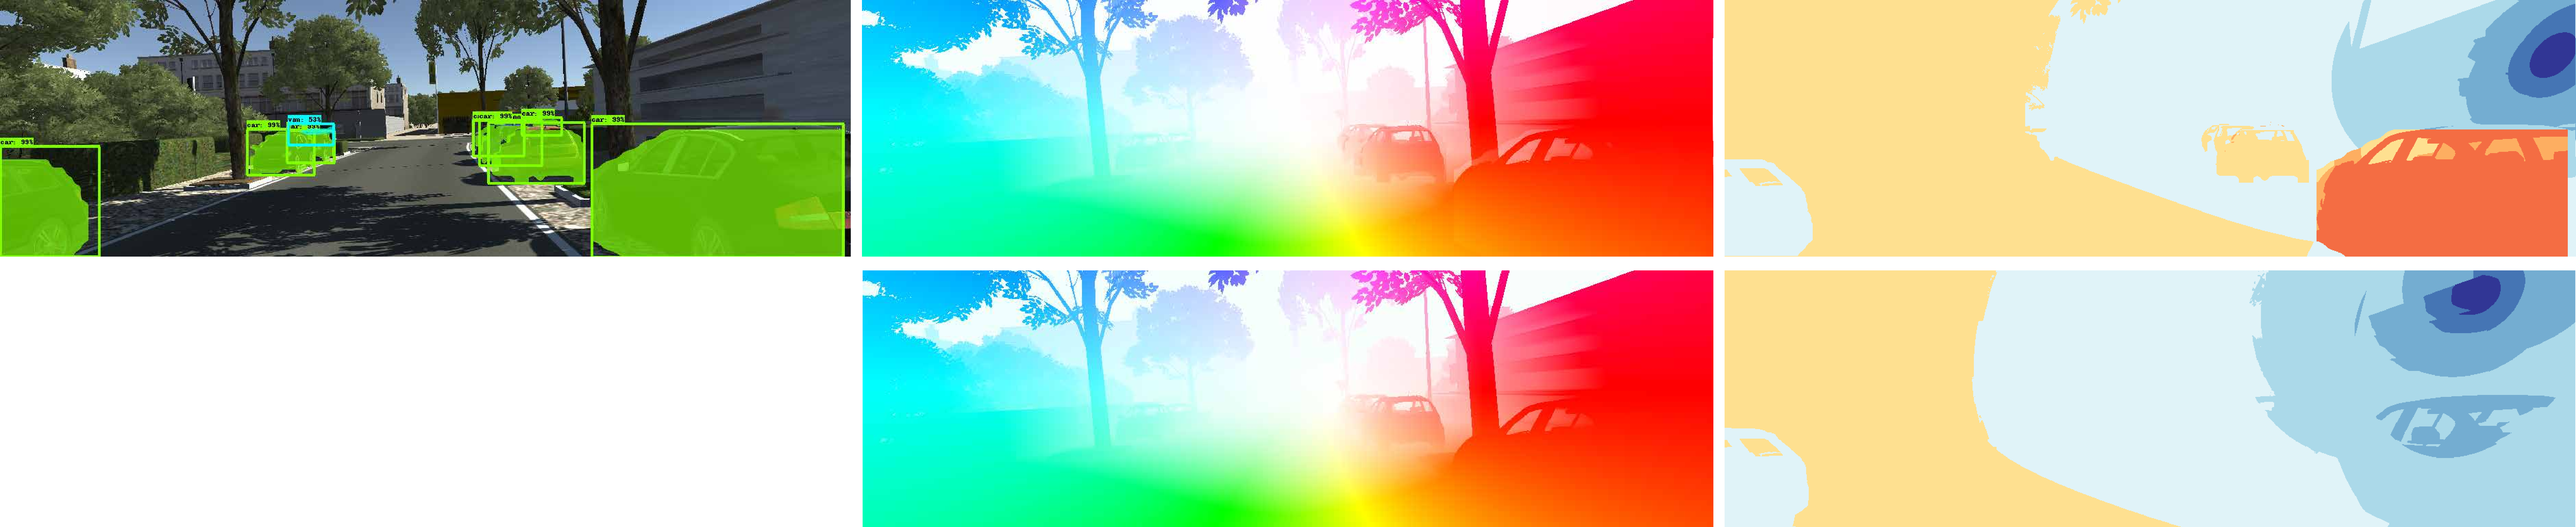
\includegraphics[width=\textwidth]{figures/moving}
\caption{
We visually compare a Motion R-CNN ResNet trained without (upper row) and
with (lower row) classifying the objects into moving and non-moving objects.
Note that in the selected example, all cars are parking, and thus the predicted
motion in the first row is an error.
From left to right, we show the first input frame with instance segmentation results as overlay,
the estimated flow, as well as the flow error map.
The flow error map depicts correct estimates ($\leq 3$ px or $\leq 5\%$ error) in blue and wrong estimates in red tones.
}
\label{figure:moving}
\end{figure}

{
\begin{table}[t]
\centering
\begin{tabular}{@{}*{10}{c}@{}}
\toprule
\multicolumn{1}{c}{Network} & \multicolumn{5}{c}{Instance Motion} & \multicolumn{2}{c}{Camera Motion} &\multicolumn{2}{c}{Flow Error} \\
  \cmidrule(lr){1-1}\cmidrule(lr){2-6}\cmidrule(l){7-8}\cmidrule(l){9-10}
FPN        & $E_{R} [deg]$ & $E_{t} [m]$ & $E_{p} [m] $ & $O_{pr}$ & $O_{rc}$  & $E_{R}^{cam} [deg]$ & $E_{t}^{cam} [m]$ & AEE   & Fl-all \\\midrule
-          & (0.279)       & (0.442)     & -            & -        & -           & (0.220)             & (0.684)           & -     &     -    \\\midrule
$\times$   & 0.301         & 0.237       & 3.331        & 0.790    & 0.916       & 0.087               & 0.053             & 11.17 & 24.91\%    \\
\checkmark & 0.293         & 0.210       & 1.958        & 0.844    & 0.914       & 0.169               & 0.050             & 8.29  & 45.22\%    \\
  \bottomrule
\end{tabular}

\caption {
Evaluation of different metrics on the Virtual KITTI validation set.
AEE: Average Endpoint Error; Fl-all: Ratio of pixels where flow estimate is
wrong by both $\geq 3$ pixels and $\geq 5\%$.
We compare network variants with and without FPN.
All metrics are averaged over all examples in the validation set.
Quantities in parentheses in the first row are the average ground truth values for the estimated
quantity. For example, we compare the error in camera angle, $E_{R}^{cam} [deg]$,
to the average rotation angle in the ground truth camera motions.
}
\label{table:vkitti}
\end{table}
}

For our initial experiments, we concatenate both RGB frames as
well as the XYZ coordinates for both frames as input to the networks.
We train both, the Motion R-CNN ResNet and ResNet-FPN variants, and supervise
camera and instance motions with 3D motion ground truth.

In Figure \ref{figure:vkitti}, we visualize instance segmentation and optical flow
results on the Virtual KITTI validation set.
In Figure \ref{figure:moving}, we visually justify the addition of the classifier
that decides between a moving and still object.
In Table \ref{table:vkitti}, we compare various metrics for the Motion R-CNN
ResNet and ResNet-FPN network variants
on the Virtual KITTI validation set.

\paragraph{Camera motion}
Both variants achieve a low error in predicted camera translation, relative to
the average ground truth camera translation. The camera rotation angle error
is still relatively high, compared to the small average ground truth camera rotation.
Although both variants use the exact same network for predicting the camera motion,
the FPN variant performs worse here, with the error in rotation angle twice as high.
One possible explanations that should be investigated in future work is
that in the FPN variant, all blocks in the backbone are shared between the camera
motion branch and the feature pyramid. In the variant without FPN, the C$5$ and
C$6$ blocks are only used in the camera branch, and thus only experience weight
updates due to the camera motion loss. This could mean that the weight updates due
to the RoI head losses are detrimental to the camera motion estimation.
As a remedy, increasing the loss weighting of the camera motion loss may be
helpful.

\paragraph{Instance motion}
The object pivots are estimated with relatively
high accuracy in both variants (given that the scenes are in a realistic scale),
although the FPN variant is significantly more
accurate, which we ascribe to the higher resolution features used in this variant.

The predicted 3D object translations and rotations still have a relatively high
error, compared to the average actual (ground truth) translations and rotations,
which may be due to implementation issues, a non-optimal network architecture,
or problems with the current 3D motion ground truth loss
(e.g., non-optimal weighting between the components of the motion loss, or between motion and classification losses).
Note that the relative error is higher for rotations, which is
also the case in the camera motion estimates.
The FPN variant is only slightly more accurate for these predictions, which again suggests
that there may still be issues with our loss design, loss weighting, or implementation, as one would expect the
FPN to yield more accurate motion estimates (as is the case for the pivot estimation).

\paragraph{Instance segmentation}
Looking at Figure \ref{figure:vkitti}, our instance segmentation results are in
some cases still lacking the accuracy seen in the Mask R-CNN Cityscapes \cite{MaskRCNN} results,
which is likely due to implementation details.
